\documentclass[10pt,landscape]{article}
\usepackage{multicol,multirow}
\usepackage{calc}
\usepackage{ifthen}
\usepackage[landscape]{geometry}
\usepackage[colorlinks=true,citecolor=blue,linkcolor=blue]{hyperref}
\usepackage[fleqn]{amsmath}
\usepackage{amssymb,amsthm,amsfonts}
\usepackage{graphicx}
\usepackage{wrapfig}
\usepackage{cancel}

\ifthenelse{\lengthtest { \paperwidth = 11in}}
{ \geometry{top=.3in,left=.3in,right=.3in,bottom=.3in} }
{\ifthenelse{ \lengthtest{ \paperwidth = 297mm}}
{\geometry{top=1cm,left=1cm,right=1cm,bottom=1cm} }
{\geometry{top=1cm,left=1cm,right=1cm,bottom=1cm} }
}
\pagestyle{empty}
\makeatletter
\renewcommand{\section}{\@startsection{section}{1}{0mm}%
{-1ex plus -.5ex minus -.2ex}%
{0.5ex plus .2ex}%x
{\normalfont\large\bfseries}}
\renewcommand{\subsection}{\@startsection{subsection}{2}{0mm}%
{-1explus -.5ex minus -.2ex}%
{0.5ex plus .2ex}%
{\normalfont\normalsize\bfseries}}
\renewcommand{\subsubsection}{\@startsection{subsubsection}{3}{0mm}%
{-1ex plus -.5ex minus -.2ex}%
{1ex plus .2ex}%
{\normalfont\small\bfseries}}
\renewcommand{\arraystretch}{1.3}
\makeatother
\setcounter{secnumdepth}{0}
\setlength{\parindent}{0pt}
\setlength{\parskip}{0pt plus 0.5ex}
\setlength{\mathindent}{0pt}
\setlength{\columnseprule}{0.2pt}
% -----------------------------------------------------------------------

\title{Partial Differential Equations}

\begin{document}
    \raggedright
    \footnotesize

    \begin{center}
        \textbf{Partial Differential Equations} \\
    \end{center}
    \begin{multicols}{3}
        \setlength{\premulticols}{1pt}
        \setlength{\postmulticols}{1pt}
        \setlength{\multicolsep}{1pt}
        \setlength{\columnsep}{2pt}

        \section{Domain and Boundary}
\begin{itemize}
    \item Domain $\Omega$ is an open subset of $\mathbb{R}^n$ (meaning all points are interior points)
    \item Boundary has to meet conditions:
    \item{ \emph{Dirichlet boundary conditions}: specify values $u$ on $\partial\Omega$: \\
        $u(x) = f(x)\ \forall x\in\partial\Omega$
    }
    \item{\emph{Neumann boundary conditions}: specify derivatives of $u$ on boundary.
    Only derivatives orthogonal to the boundary give additional information: \\
    normal derivative: $\frac{\partial u}{\partial n} = g(x)\ \forall x\in\partial\Omega$
    }
\end{itemize}

        \section{Classification}\label{sec:classification}
\begin{center}
    \makebox[\columnwidth]{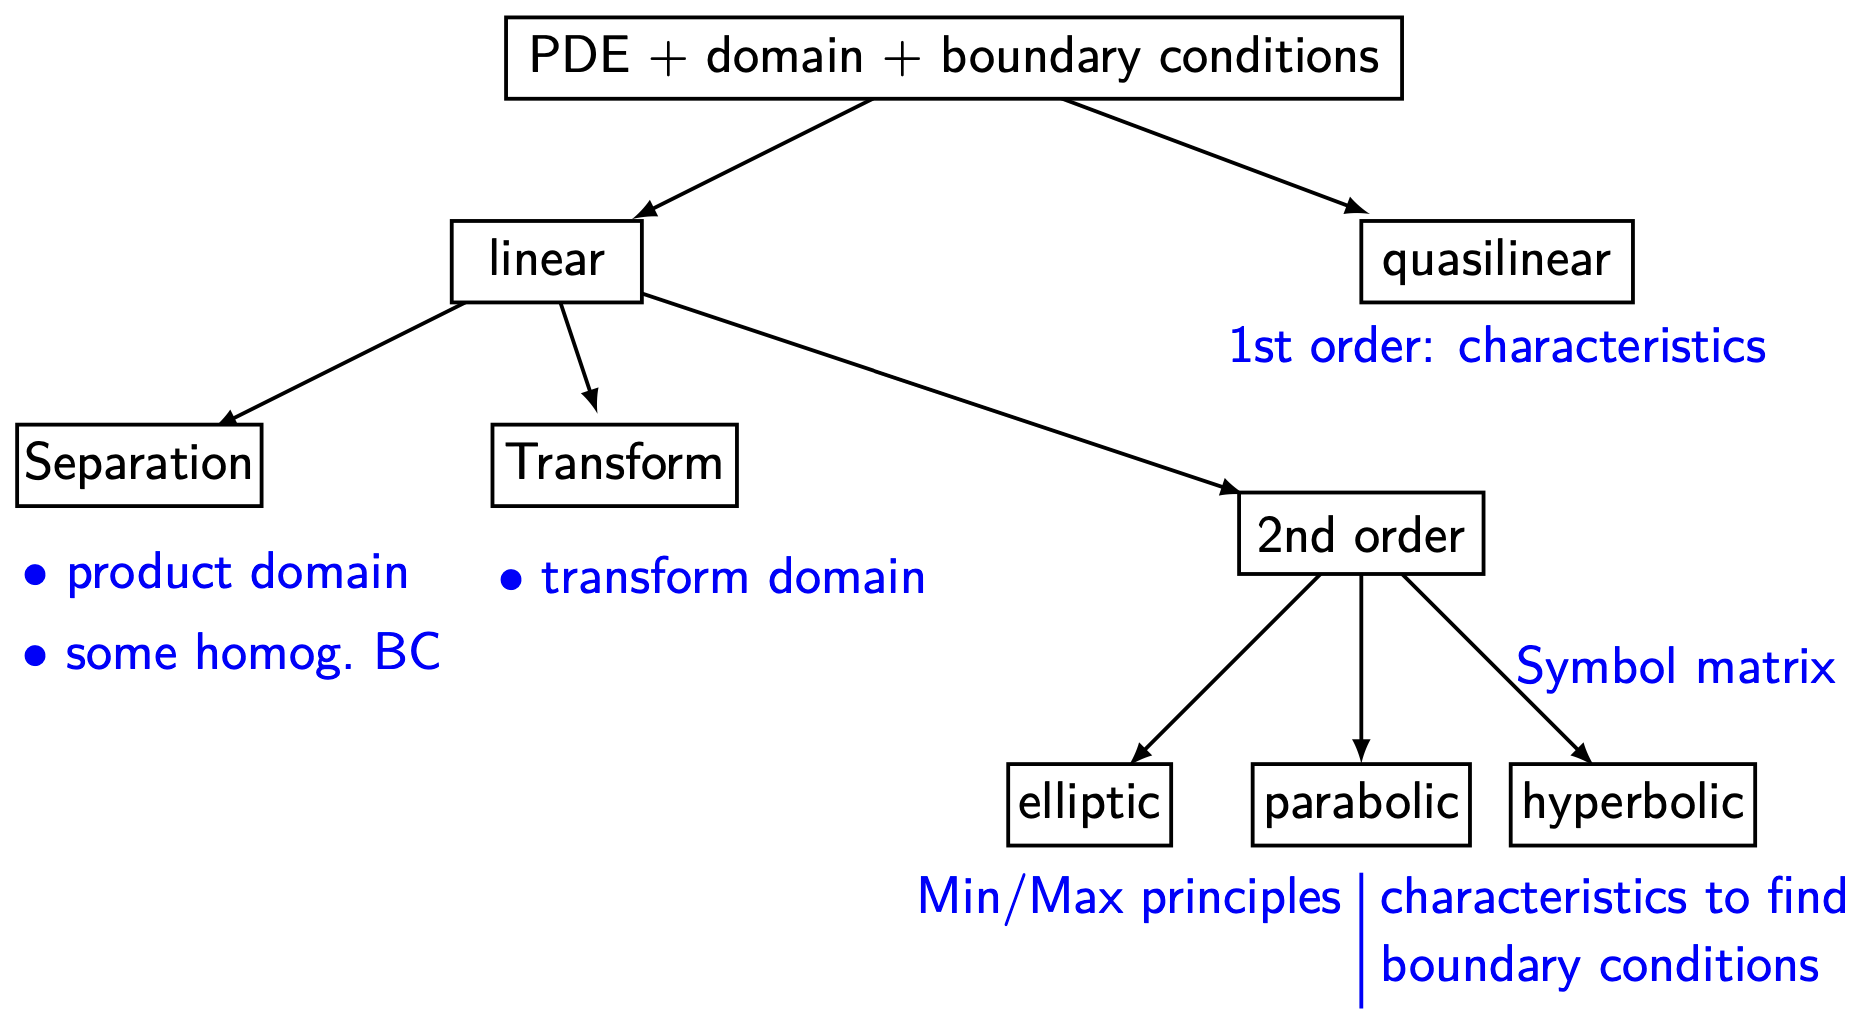
\includegraphics[width=0.9\columnwidth]{images/decision-tree}}
\end{center}

\subsection{Linearity}\label{subsec:linearity}
Given an equation involving a function $u(x), x\in\mathbb{R}$ and its derivatives,
there is a function $F$ describing the relation:
\begin{align*}
    F\left(
    \begin{matrix}
        x,y,z,p,q,s,t,r,\ldots                         \\
        \downarrow \text{(corresponding to)}\downarrow \\
        x, y, u, \frac{\partial u}{\partial x}, \frac{\partial u}{\partial y}, \frac{\partial^2 u}{\partial x^2},
        \frac{\partial^2 u}{\partial x\partial y},\frac{\partial^2 u}{\partial y^2}, \ldots
    \end{matrix}
    \right) = 0
\end{align*}
(common variable names $p_i\rightarrow\frac{\partial u}{\partial x_i}$ and
$t_{ij} \rightarrow\frac{\partial^2 u}{\partial x_i\partial x_j}$)

A PDE is \emph{linear} when function $F$ is linear in $u,p_1,\ldots,p_n,t_{11},\ldots,t_{nn},\ldots.$

A PDE is \emph{quasilinear} when function $F$ is linear in $p_1,\ldots,p_n,t_{11},\ldots,t_{nn},\ldots.$

For example, given the heat equation $u_t=\kappa u_{xx}$, $F$ would be $F(p_1,t_{22})=p_1-\kappa t_{22}$.

\symbolicsubsection{2\textsuperscript{nd} Order PDEs: Symbol Matrix}

The symbol matrix of the 2\textsuperscript{nd} order partial differential operator

\begin{align*}
    L=\sum_{i,j=1}^{n}a_{ij}(x)\frac{\partial^2}{\partial x_i \partial x_j}+\sum_{i=1}^n b_i(x)\frac{\partial}{\partial x_i}+c(x)
\end{align*}

is the symmetric matrix

\begin{align*}
    A=
    \begin{bmatrix}
        a_{11} & a_{12} & \ldots & a_{1n} \\
        a_{21} & a_{22} & \ldots & a_{2n} \\
        \vdots & \vdots & \ddots & \vdots \\
        a_{n1} & a_{n2} & \ldots & a_{nn}
    \end{bmatrix}
\end{align*}

For example:

\begin{center}
    \makebox[\columnwidth]{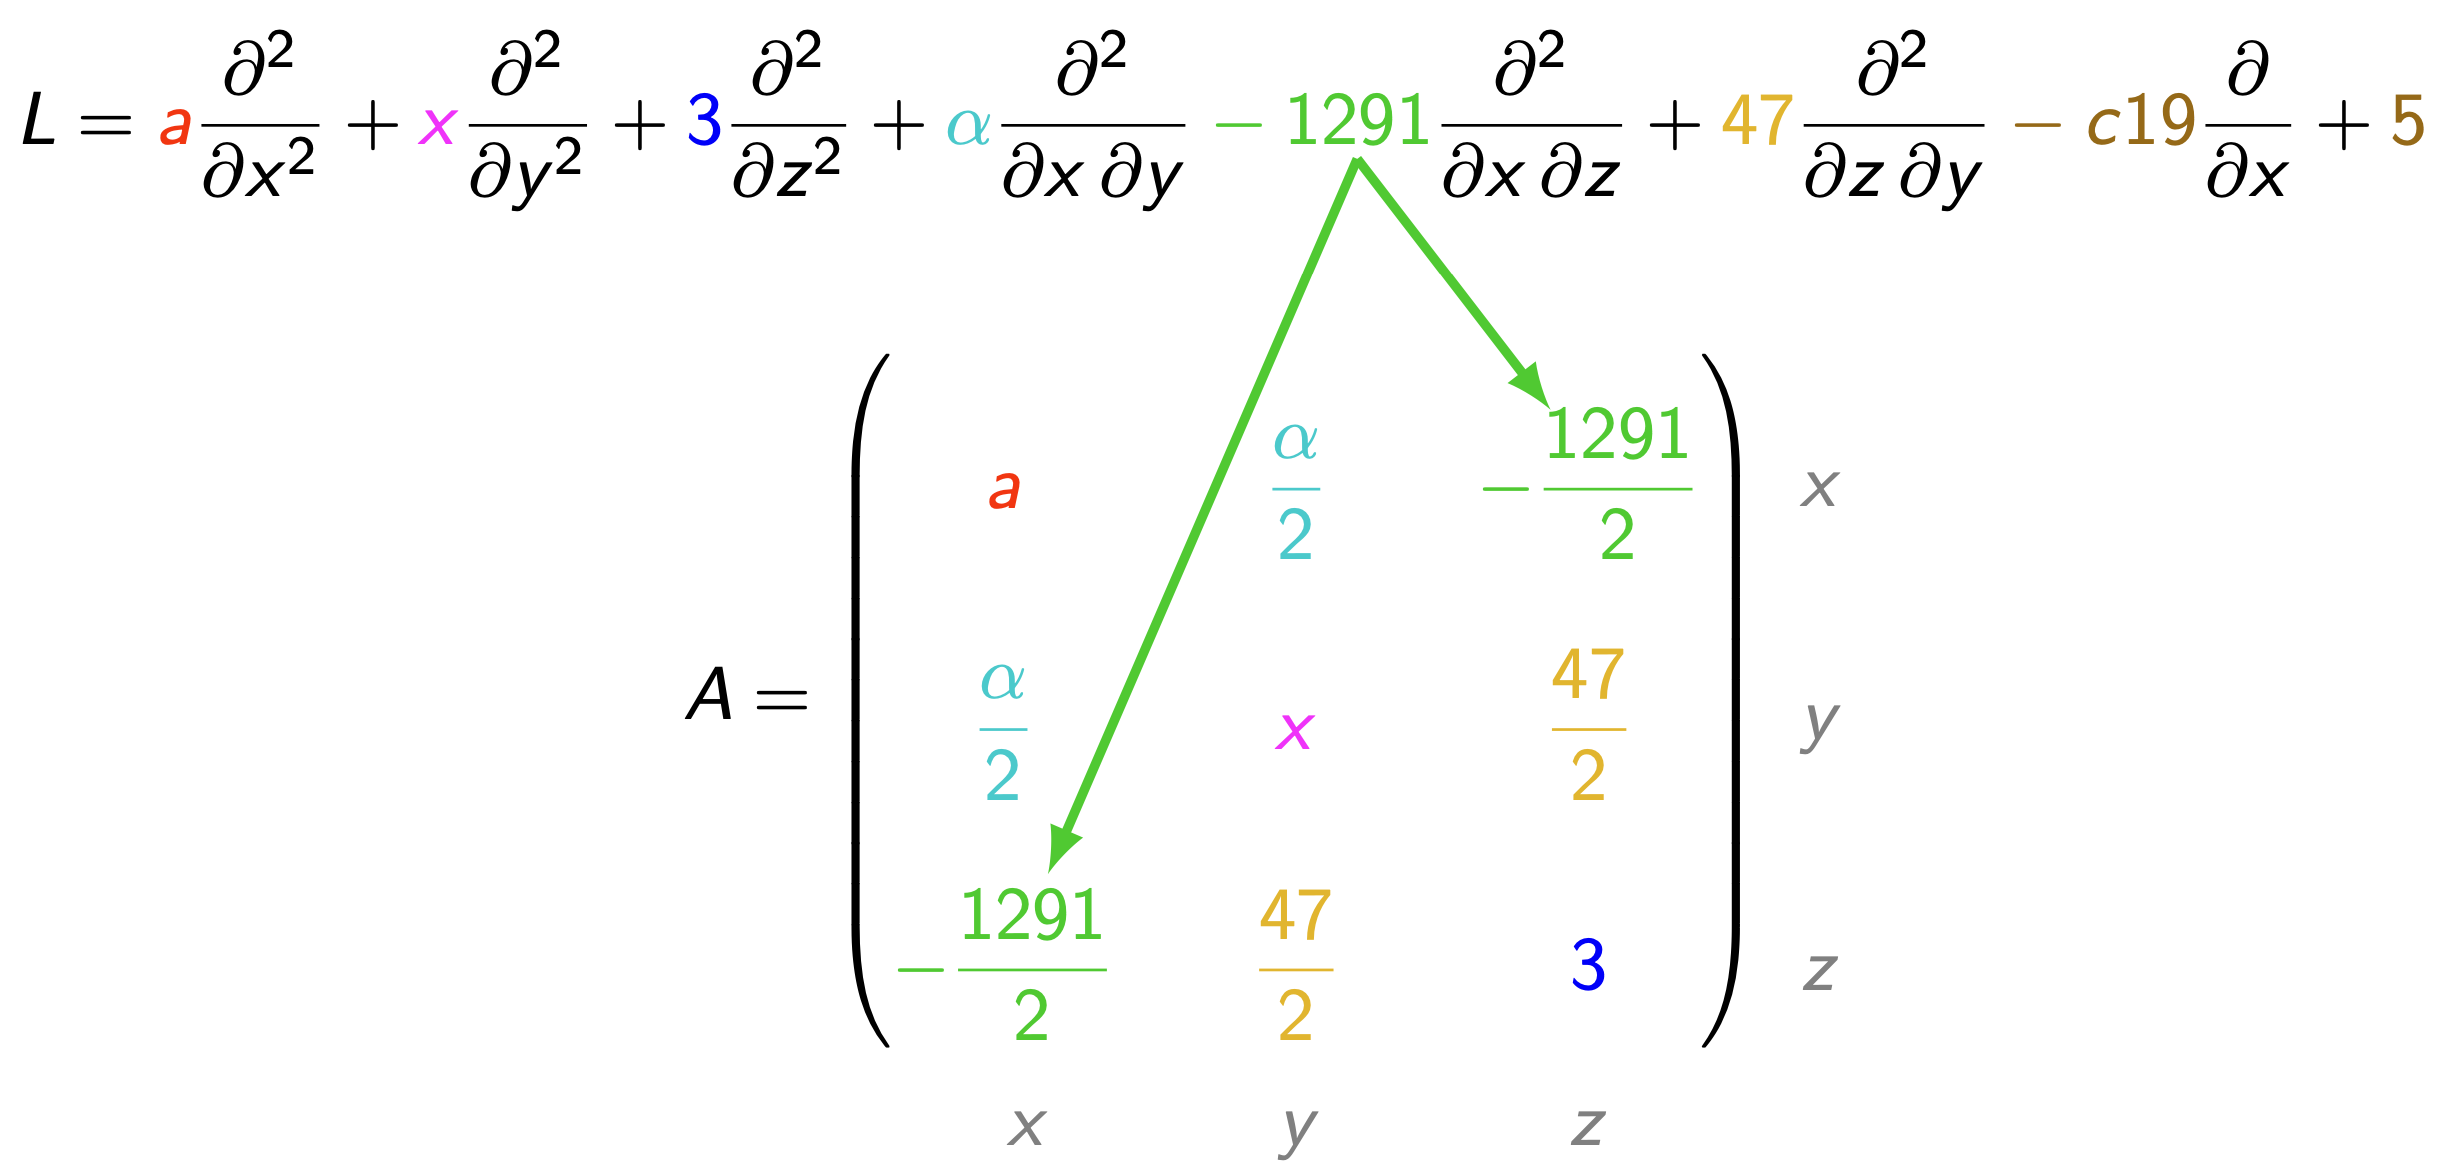
\includegraphics[width=0.9\columnwidth]{images/symbol-matrix}}
\end{center}

The type of equation can be inferred by the sign of the eigenvalues $\lambda_1,\ldots,\lambda_n$ of the symbol matrix.
Calculating the determinant ($\det A=\prod_i \lambda_i$) and trace ($\mathrm{tr}\ A=\sum_i \lambda_i$)
reveals information about the signs of its eigenvalues:

\subsubsection{Two Variables of PDE}

\begin{align*}
    \det A
    \left\{
    \begin{matrix}
        >0 & \text{elliptic (eigenvalues have same sign)}       \\
        =0 & \text{parabolic (at least one eigenvalue is zero)} \\
        <0 & \text{hyperbolic (eigenvalues have opposite sign)}
    \end{matrix}
    \right.
\end{align*}

\subsubsection{Three Variables of PDE}

\begin{align*}
    \mathrm{rank}\ A < 2 & \Rightarrow \text{not classified} \\
    \det A\text{ and }\mathrm{tr}\ A\text{ have different sign} & \Rightarrow\text{hyperbolic} \\
    \det A=0\text{, semidefinite (Cholesky decomp.)} & \Rightarrow\text{parabolic} \\
    A\text{ or }-A\text{ positive definite (Cholesky)} & \Rightarrow\text{elliptic} \\
    \text{all other cases} & \Rightarrow\text{hyperbolic}
\end{align*}

        \section{Quasilinear PDEs}\label{sec:quasilinear-pdes}

\subsection{Characteristics}\label{subsec:characteristics}

\begin{wrapfigure}{r}{0.4\columnwidth}
    \centering
    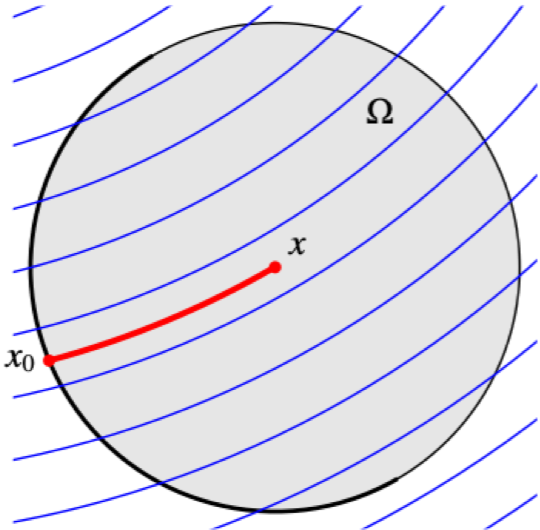
\includegraphics[width=0.4\columnwidth]{images/quasilinear}
\end{wrapfigure}

The PDE

\begin{align*}
    a(x,y,u)\frac{\partial u}{\partial x}+b(x,y,u)\frac{\partial u}{\partial y} = c(x,y,u)
\end{align*}

can be written in vector notation:

\begin{align*}
{\color{green}
\underbrace{
    \begin{pmatrix}
        a(x,y,u) \\
        b(x,y,u) \\
        c(x,y,u)
    \end{pmatrix}
}_{\vec t}
}
    \cdot
    {\color{black}
    \underbrace{
        \begin{pmatrix}
            \frac{\partial u}{\partial x} \\
            \frac{\partial u}{\partial y} \\
            -1
        \end{pmatrix}
    }_{\vec{n}}
    }
    &= 0
\end{align*}

where $\color{black}\vec{n}$ is a normal vector and $\color{green}\vec{t}$ is always tangential to the solution surface.
Therefore, we can elaborate a solution algorithm:
\begin{enumerate}
    \item{
        Using the Cauchy initial curve, we formulate
        \begin{align*}
            \vec{v}(s) = \begin{pmatrix}
                             v_x({\color{red}s} ) & v_y({\color{red}s}) & v_z({\color{red}s})
            \end{pmatrix}^T
        \end{align*}
        which is a point on the initial curve, parameterised by $s$.
    }
    \item{
        Find characteristic curves as solution of the ODEs

        \begin{align*}
            \frac{d}{d{\color{blue}t}}
            \begin{bmatrix}
                x({\color{blue}t}, {\color{red}s}) \\
                y({\color{blue}t}, {\color{red}s}) \\
                z({\color{blue}t}, {\color{red}s})
            \end{bmatrix}
            =
            \begin{bmatrix}
                a(x({\color{blue}t},{\color{red}s}), y({\color{blue}t},{\color{red}s}), z({\color{blue}t}, {\color{red}s})) \\
                b(x({\color{blue}t},{\color{red}s}), y({\color{blue}t},{\color{red}s}), z({\color{blue}t}, {\color{red}s})) \\
                c(x({\color{blue}t},{\color{red}s}), y({\color{blue}t},{\color{red}s}), z({\color{blue}t}, {\color{red}s}))
            \end{bmatrix}
        \end{align*}
        with
        \begin{align*}
            \begin{bmatrix}
                x({\color{blue}0}, {\color{red}s}) \\
                y({\color{blue}0}, {\color{red}s}) \\
                z({\color{blue}0}, {\color{red}s})
            \end{bmatrix}
            =
            \vec{v}({\color{red}s})
            =
            \begin{bmatrix}
                v_x({\color{red}s} ) \\
                v_y({\color{red}s})  \\
                v_z({\color{red}s})
            \end{bmatrix}
        \end{align*}
    }
    \item{
        Eliminate the variables {\color{blue}t} and {\color{red}s} and condense solution into a function $u(x, y)$:
        \begin{align*}
            \left.
            \begin{matrix}
                x=x({\color{blue}t},{\color{red}s}) \\
                y=y({\color{blue}t},{\color{red}s}) \\
                u=z({\color{blue}t},{\color{red}s})
            \end{matrix}
            \ \ \right\}
            \ u=u(x,y)
        \end{align*}
    }
\end{enumerate}

        \section{Linear PDEs}\label{sec:linear-pdes}
        \symbolicsubsection{Separation}\label{subsec:separation}
Conditions, when separation may be successful:

\begin{itemize}
    \item Homogeneous, linear PDE
    \item Homogeneous boundary conditions
    \item Domain must be a cartesian product (i.e. some form of rectangle when in cartesian coordinate system)
\end{itemize}

if these are given, we can try:

\begin{enumerate}
    \item Assume the structure of the solution to be in the form of some ansatz with separable variables, usually a product $u(x,y)=X(x)\cdot Y(y)$
    \item{
        Substitute $u$ in PDE with ansatz by variable:
        \begin{align*}
            \text{all terms of }x = \text{all terms of }y = {\color{red}\lambda}
        \end{align*}
        and solve the ordinary differential equations for $X(x)$ and $Y(y)$.
    }
    \item Use \emph{homogeneous} boundary conditions to determine admissible values ${\color{red}\lambda}_k$.
    \item Solve equations: $X_k(x)$ and $Y_k(y)$ $\Rightarrow u_k(x,y)=X_k(x)\cdot Y_k(y)$ using ansatz.
    \item Combine solutions: $u(x,y)=\sum_{k\in \mathbb{Z}}\left(a_ku_k(x,y)\right)$
    \item Use remaining boundary conditions to determine $a_k$.
\end{enumerate}

\paragraph{Separation Example}

Given the wave equation $\frac{\partial^2u}{\partial t^2}=\frac{\partial^2 u}{\partial x^2}$
for a string mounted between $u(0,t)=u(\pi,t)=0$ and is in the rest position at $t=0$: $u(x,0)=0$ but has initial velocity
$\frac{\partial u}{\partial t}(0,x)=\sin^3(x)=\frac{3}{4}\sin x-\frac{1}{4}\sin 3x$.
We choose the Ansatz $u(x,t)=X(x)T(t)$:

\begin{align*}
    \begin{matrix}
        X(x)T''(t)=X''(x)T(x) & |\div X(x)T(t) \\
        T''(t)\div T(t) = X''(x)\div X(x) = \mu
    \end{matrix} \\
\end{align*}
Hence, we receive the ODEs

\begin{align*}
    \mu T(t) = T''(t) \\
    \mu X(x) = X''(x)
\end{align*}
with $\mu < 0$ to receive oscillating solutions, the ODEs have the solutions

\begin{align*}
    X(x) & = C \sin(\sqrt\mu x)+\cancel{ D\cos(\sqrt\mu x) } \\
    T(t) & = A \sin(\sqrt\mu t)+B \cos(\sqrt\mu t)
\end{align*}
by taking into account the boundary conditions $X(0)=X(\pi)=0$, yielding $C=1,D=0$ and $\sqrt{n}\in\mathbb{N}$.
Therefore, we have the general solution
\begin{align*}
    u(x,t) & = \sum_{n=1}^\infty \sin(nx)\cdot\left( A_n\sin(nt)+B_n\cos(nt) \right) \\
    \ & = \sum_{n=1}^\infty A_n\sin(nx)\sin(nt) + \sum_{n=1}^\infty B_n\sin(nx)\cos(nt)
\end{align*}

considering the boundary conditions:
\begin{align*}
    u(x,0) = 0 = \sum_{n=1}^\infty B_n\sin(nx)\underbrace{\cos(0)}_{=1} \Rightarrow B_n=0
\end{align*}
and

\begin{align*}
    \ & \frac{\partial u}{\partial t} = \sum_{n=1}^\infty nA_n\sin(nx)\cos(nt)\\
    \ & \rightarrow \frac{\partial u}{\partial t}(x,0) = \sum_{n=1}^\infty nA_n\sin(nx) = \frac{3}{4}\sin x-\frac{1}{4}\sin 3x \\
    \ & \Rightarrow A_1=3/4, A_3=-1/12, A_{n\setminus \{1,3\}}=0 \\
    \ & \Rightarrow u(x,t)=(3/4)\sin(x)\sin(t)-(1/12)\sin(3x)\sin(3t)
\end{align*}

        \subsection{Transformation}\label{subsec:transformation}
\begin{enumerate}
    \item{
        Transform equation: derivatives turn into algebraic expressions:
        \begin{align*}
            \left(
            \mathcal{L}\frac{\partial u(t,y)}{\partial t}
            \right)(s) =
            s
            \underbrace{(\mathcal{L}f)(s, y)}_{=y_s(y)}
            -u(0,y)
        \end{align*}
    }
    \item{
        Transform y-boundary conditions: gives boundary conditions for
        \begin{align*}
            u(t,0) & =g(t) \\
            y_s(0)=(\mathcal{L}u(t,0))(s) & = (\mathcal{L}g)(s)
        \end{align*}
    }
    \item Solve PDE with fewer derivatives, ODEs
    \item Inverse transform
\end{enumerate}

\subsubsection{Laplace Transform}

(Only works on linear equations.)
The Laplace transform of a function $f:\mathbb{R}^+\to \mathbb{R}$ is the function

\begin{align*}
    \mathcal{L}f : \mathbb{R}^+\to \mathbb{R} : s \rightarrowtail \mathcal{L}f(s) = \int_0^\infty f(t)e^{-st}\ dt
\end{align*}

It is linear:

\begin{align*}
	\mathcal{L}(\alpha f+\beta f)=\alpha\mathcal{L}f+\beta\mathcal{L}f
\end{align*}

Example transformations:
\begin{align*}
	\begin{matrix}
		\text{Constant: } & \text{Exponential: } & \text{Derivative: } \\
		f(t)=c & f(t)=e^{-ct} & f(t)=g^{(n)}(t) \\
		(\mathcal{L}f)(s) = \frac{c}{s} & (\mathcal{L}f)(s) = \frac{1}{c+s} & (\mathcal{L}f^{(n)})(s)= \\
		& & -f^{(n-1)}(0)+s\left(\mathcal{L}f^{(n-1)}\right)(s) \\
		& & \text{(removes t-derivatives: }\frac{\partial}{\partial t}\rightarrow s\text{)}
	\end{matrix}
\end{align*}

\subsubsection{Fourier Transform}

For $f : \mathbb{R}\to\mathbb{C} : x \rightarrowtail f(x)$ the Fourier transform of $f$ is defined as

\begin{align*}
    \mathcal{F}f = \hat{f} : \mathbb{R}\to\mathbb{C} : k\rightarrowtail
    \frac{1}{\sqrt{2\pi}}\int_{-\infty}^{\infty}f(x)e^{-ikx}\ dx
\end{align*}

It turns the derivative $\frac{\partial}{\partial x}$ into a multiplication by $-ik$ (second derivatives are reduced to $i^2=-1$):
\begin{align*}
	(\mathcal{F}f^{(n)})(k) = (ik)^n\mathcal{F}f(k)
\end{align*}

The function $f$ can be recovered from $\hat{f}$ by
\begin{align*}
    f(x)=(\mathcal{F}^{-1}\hat{f})(x)
    = \frac{1}{\sqrt{2\pi}}\int_{-\infty}^\infty \hat{f}(k) e^{ikx}\ dk
\end{align*}

        \section{PDEs of Second Order}

Linear PDEs of second order have the form
\begin{align*}
	\sum_{i,j=1}^n a_{ij}\frac{\partial ^2}{\partial x_i\partial x_j}u+\sum_{i=1}^nb_i\frac{\partial}{\partial x_i}u + cu = f
\end{align*}

The equations fall into these categories:
\emph{Elliptic} (potential problem), \emph{parabolic} (heat equation, diffusion)
and \emph{hyperbolic} (wave equation, linearised supersonic flow).

\symbolicsubsection{Splitting the Solution}

Given a second order linear differential operator $L$,
we have the PDE $Lu = f \text{ in }\Omega$ with $u = g \text{ on }\partial\Omega$.

\begin{enumerate}
	\item We try to find a particular solution {\color{blue}$Lu_p = f$ in $\Omega$}, satisfying only the PDE and neglecting boundary conditions
	\item{
		To solve the original problem,
		we need an additional summand $u_r$ taking care of boundary values to receive the solution $u_p + u_r$.
		However, $u_r$ still needs to solve the PDE but due to linearity, this reduces to a homogeneous problem:
		\begin{align*}
			L(u_p + u_r) = f + Lu_r = f \Rightarrow{\color{blue} Lu_r = 0\text{ in }\Omega}
		\end{align*}
	}
	\item{
		Ensure that the boundary conditions are satisfied:
		\begin{align*}
			u_p+u_r = g \Rightarrow {\color{blue}u_r = g - u_p\text{ on }\partial\Omega}
		\end{align*}
	}
	\item{
		If the solution is not unique, we're able to find other solutions using an additional term $u_h$:
		\begin{align*}
			L(u_p + u_r + u_h) = f + Lu_h &\ \Rightarrow Lu_h = 0\text{ in }\Omega \\
			u_p + u_r + u_h = g + u_h &\ \Rightarrow u_h = 0\text{ on }\partial\Omega
		\end{align*}
	}
\end{enumerate}

For example, consider the PDE $\nabla^2 u = 4$ in $\Omega = \{(x,y)\ |\ x^2 + y^2 < 1\}$ and $u = 0.5x+0.5$ on $\partial\Omega$.
This has the particular solution $u_p(x,y)=x^2+y^2$.
To fix boundary conditions, we find a solution $u_r$ of the homogeneous problem with boundary values
$u_r = 0.5x + 0.5 - u_p(x,y) = 0.5x + 0.5 - \underbrace{1}_{\text{on }\partial\Omega} = 0.5x - 0.5$ giving the complete solution
$u(x,y) = u_p(x,y) + u_r(x,y) = x^2 + y^2 + 0.5x - 0.5$.


        \section{Numerical Methods}
\subsection{Discretisation of Operators}

\begin{align*}
	\frac{\partial g}{\partial x}
	\approx
	\frac{g(x + \Delta x) - g(x)}{\Delta x}
\end{align*}

\begin{align*}
	\frac{\partial^2 g}{\partial x^2}
	\approx
	\frac{g(x + \Delta x) - 2\cdot g(x) + g(x - \Delta x)}{\Delta x^2}
\end{align*}

($\Delta$ referring to step size)
\subsection{Finite Elements}

We have a set of given local basis functions $v_1(x), \ldots, v_n(x)$ that are continuous and piecewise differentiable.
We subdivide $\Omega$ into meshes and assign each nodal point a nodal variable $a_k$.
Then, we use shape functions to represent the PDE on the mesh,
e.g. using triangular functions $l_1(x)=1-x$ and $l_2(x) = x$ to obtain \emph{local} element matrices
\begin{align*}
	E = 
	\begin{bmatrix}
		\int_0^1 l_1^\prime(s)\cdot l_1^\prime(s)\ ds & \int_0^1 l_1^\prime(s)\cdot l_2^\prime(s)\ ds \\
		\int_0^1 l_2^\prime(s)\cdot l_1^\prime(s)\ ds & \int_0^1 l_2^\prime(s)\cdot l_2^\prime(s)\ ds
	\end{bmatrix}
	=
	\begin{bmatrix}
		1 & -1 \\
		-1 & 1
	\end{bmatrix}
\end{align*}

that can then be used to construct the mesh matrix $M=1/h\cdot E$ using mesh size $h$.
Afterwards, the global Ritz matrix can be computed, e.g. for a one-dimensional mesh with 4 nodal points and 2 unknown inner points,
yielding 4 base functions $v_1,v_2,v_3,v_4$:

\begin{align*}
	R^4 = \begin{bmatrix}
		{\color{red} M^{(1)}_{0,0}} & \color{red}{M^{(1)}_{0,1}} & 0 & 0 \\
		{\color{red} M^{(1)}_{1,0}} & {\color{red} M^{(1)}_{1,1}} + {\color{blue} M^{(2)}_{0,0}} & {\color{blue} M^{(2)}_{0,1}} & 0 \\
		0 & {\color{blue} M^{(2)}_{1,0}} & {\color{blue} M^{(2)}_{1,1}} + {\color{green} M^{(3)}_{0,0}} & {\color{green} M^{(3)}_{0,1}} \\
		0 & 0 & {\color{green} M^{(3)}_{1,0}} & {\color{green} M^{(3)}_{1,1}}
	\end{bmatrix}
\end{align*}

The system vector can then be calculated:

\begin{align*}
	\vec{r^4} = \begin{pmatrix}
		\int_0^1 f(x)\cdot v_0(x)\ dx \\
		\vdots \\
		\int_0^1 f(x)\cdot v_3(x)\ dx
	\end{pmatrix}
\end{align*}

Finally, we have obtained the Ritz system: $R^4\cdot\vec{a}=\vec{r^4}$.
That yields the approximation function (as defined by the ansatz): $\tilde{u}(x)=\sum_{i=0}^3 a_i\cdot v_i(x)$
3with $a_0$ and $a_3$ fulfilling the boundary conditions.
        \newpage
        \section{Cheat Sheet}
\subsection{Roots}

\begin{align*}
	\sqrt[n]{a}\cdot\sqrt[n]{b} & = \sqrt[n]{a\cdot b} \\
	\frac{\sqrt[n]{a}}{\sqrt[n]{b}} & = \sqrt[n]{\frac{a}{b}} \\
	(\sqrt[n]{a})^m & = \sqrt[n]{a^m} \\
	\sqrt[m]{\sqrt[n]{a}} & = \sqrt[m\cdot n]{a}
\end{align*}


\subsection{Logarithm}

\begin{align*}
	\log_n(a\cdot b) & = \log_n(a) + \log_N(b) \\
	\log_n(a\div b) & = \log_n(a) - \log_N(b) \\
	\log_n(a^b) & = b \cdot \log_n(a)
\end{align*}

\subsection{Trigonometry}

\begin{align*}
	\tan\theta & = \frac{\sin\theta}{\cos\theta} \\
	\sin -\theta & = -\sin\theta\text{ (cos same)} \\
	\sin 2\theta & = 2\sin\theta\cos\theta \\
	\cos 2\theta & = 2\cos^2\theta - \sin^2\theta = 2\cos^2\theta - 1 = 1 - 2\sin^2\theta \\
	\sin(\alpha \pm \beta) & = \sin\alpha\cos\beta\pm\cos\alpha\sin\beta \\
	\cos(\alpha\pm\beta) & = \cos\alpha\cos\beta \mp \sin\alpha\sin\beta \\
	\sinh x & = \frac{e^x - e^{-x}}{2}=\frac{e^{2x}-1}{2e^x} \\
	\cosh x & = \frac{e^x + e^{-x}}{2} = \frac{e^{2x}+1}{2e^x} \\
	\tanh x & = \sinh x \div \cosh x \\
	\coth x & = \cosh x \div \sinh x \\
	\mathrm{sech}\ x & = 1 \div \cosh x = 2 \div (e^x+e^{-x})
\end{align*}

\subsection{Derivatives}
\begin{tabular}{r|l}
	$f(x)$ & $\frac{df}{dx}$ \\
	\hline
	$\sinh(x)$ & $\cosh(x)$ \\
	$\cosh(x)$ & $\sinh(x)$ \\
	$\mathrm{arcsinh}(x)$ & $1 \div \sqrt{x^2+1}$ \\
	$\mathrm{arccosh}(x)$ & $1 \div \sqrt{x^2 - 1}$ ($1<x$) \\
	$\tan(x)$ & $\cos^{-2}(x)$ \\
	$\log(x)$ & $x^{-1}$
\end{tabular}

\subsection{Integrals}
\begin{tabular}[h]{rl}
	$\int x^n\ dx$ & $= \frac{1}{n+1}x^{n+1} + C$ \\
	$\int \frac{1}{x}\ dx$ & $= \ln |x| + C$ \\
	$\int \frac{1}{ax + b}\ dx$ & = $\frac{1}{a} \ln |ax+b| + C$ \\
	$\int \frac{1}{(x+a)^2}\ dx$ & $= -\frac{1}{x+a} + C$ \\
	$\int \frac{1}{1 + x^2}$ & $= \tan^{-1} x + C$ \\
	$\int \ln ax\ dx$ & $= x\ln ax - x + C$ \\
	$\int e^{ax}\ dx$ & $= \frac{1}{a} e^{ax} + C$ \\
	$\int \sin(ax)\ dx$ & $= -\frac{1}{a}\cos(ax) + C$ \\
	$\int \sin^2(ax)\ dx$ & $= \frac{x}{2}-\frac{\sin(2ax)}{4a} + C$ \\
	$\int x\cos x\ dx$ & $= \cos x + x\sin x + C$ \\
	$\int \sinh(ax)\ dx$ & $= a^{-1}\cosh{ax} + C$ \\
	$\int \cosh(ax)\ dx$ & $= a^{-1}\sinh{ax} + C$ \\
\end{tabular}

\subsection{Integration Techniques}
\subsubsection{Integration by Parts}
\begin{equation*}
	\int_a^b u(x)v'(x)\ dx = \left[ u(x)v(x) \right]_a^b-\int_a^bu'(x)v(x)\ dx
\end{equation*}

Or, with $u=u(x)$, $du=u'(x)\ dx$, $v=v(x)$ and $dv=v'(x)\ dx$:
\begin{equation*}
	\int u\ dv=uv - \int v\ du
\end{equation*}

\subsubsection{Substitution}
\begin{equation*}
	\int_a^b f(g(x))\cdot g'(x)\ dx = \int_{g(a)}^{g(b)}f(u)\ du
\end{equation*}

\subsubsection{Leibniz Integral Rule}
\begin{multline*}
	\frac{d}{dx}\left(\int_{a(x)}^{b(x)}f(x,t)\ dt\right)
	=
	\\
	f(x,b(x))\cdot\frac{d}{dx}b(x)
	-f(x,a(x))\cdot\frac{d}{dx}a(x)
	+\int_{a(x)}^{b(x)}\frac{\partial}{\partial x}f(x,t)\ dt
\end{multline*}
Special case where $a(x)=a=\mathrm{const.}$ and $b(x)=b=\mathrm{const.}$:
\begin{equation*}
	\frac{d}{dx}\left(\int_a^b f(x,t)\ dt\right)
	=\int_a^b\frac{\partial}{\partial x}f(x,t)\ dt
\end{equation*}

\subsection{Particular Solutions to Simple ODEs}

\begin{tabular}[h]{rcl}
	$f'(x)=\frac{c}{x}f(x)$ & $\Rightarrow$ & $f(x)=k_1y^c$ \\
	$f'(x)=x\cdot f(x)$ & $\Rightarrow$ & $f(x)=k_1e^{cx}$ \\
	$f''(x) = c\cdot f(x)$ & $\Rightarrow$ & $f(x) = k_1e^{\sqrt{c}x}+k_2e^{-\sqrt{c}x}$ \\
	$f''(x) = -c\cdot f(x)$ & $\Rightarrow$ & $f(x)=k_1\sin(\sqrt{c}x)+k_2\cos(\sqrt{c}x)$ \\
	$f'(x)+af(x) = b$ & $\Rightarrow$ & $f(x) = \left(f(0)-\frac{b}{a}\right)e^{-ax}+\frac{b}{a}$
\end{tabular}

\subsection{Harmonic Function}

A function is harmonic if it fulfils $\Delta f = 0$. The mean value property applies:
\begin{align*}
	u(x) = \frac{1}{\mu(S_r(x))}\int_{S_r(x)}u(y)\ d\mu(y)
\end{align*}

\subsection{Polar Coordinates}
\begin{align*}
	x = r\cos \varphi \\
	y = r\sin \varphi
\end{align*}

The Laplace operator in polar coordinates is
\begin{align*}
	\Delta u = \frac{1}{r}\frac{\partial}{\partial r}
	\left(r\frac{\partial u}{\partial r}\right)
	+\frac{1}{r^2}\frac{\partial^2 u}{\partial \varphi^2}
\end{align*}
    \end{multicols}
\end{document}
